\documentclass[12pt]{article}

\usepackage[top=50pt, bottom=50pt, left=90pt, right=90pt]{geometry}
\usepackage[pdftex]{graphicx}
\usepackage{soul}

\usepackage{lipsum}%% a garbage package you don't need except to create examples.
\usepackage{fancyhdr}
\pagestyle{fancy}

%This is some header and footer information
\lfoot{Kids Coding Club}
\rfoot{\thepage}
\cfoot{}
\renewcommand{\headrulewidth}{0pt}
\renewcommand{\footrulewidth}{0.4pt}

%Basic title information about original author and title
\title{Class 3 - X-Wing Project / Lists}
\author{Tyler Bounds}
\date{\today}
 

\begin{document}

\maketitle


\section *{Introduction to the Project}
	\begin{itemize}
		\item This project is designed mainly to teach Scratch's list data type. This project will also cover how to remix a project as well as how to use someone else's project in their own, with proper crediting. 

		\item The first step is to have the students remix the \textbf{XWing Kids Coding Club} project. They can either just search the project name from Scratch's main page or search for my studio \textbf{tbounds42}. 

		\item Click the project, then \textbf{See inside}, and then click \textbf{remix}, the orange button in the top-right. 

		\item After they have remixed it, walk them through the high-level details of the project. 

		\begin{itemize}
    		\item{Stage - Contains the backdrop as well as the scripts for animating the backdrop.}
    		\item{X-Wing - This is the player. They can move and shoot currently.}
    		\item{Laser - This is the projectile the player fires. It collides with the enemies.}
    		\item{Tie Fighter - This is the enemy that spawns at the top, flies straight to the bottom, and dies to the lasers.}
    		\item{Gem - This is currently just a sprite with a collection of various gem costumes.}
    		\item{UI - This is just a floating sprite meant to hold the text for the scores.}
		\end{itemize}
	
	\end{itemize}



\section *{Introduction to Lists}
	\begin{itemize}
		\item Lists are exactly what like what they sound like, a list. Think grocery list, or attendance list, or Christmas list. They are containers for data that are stored in sequential order. 

		\item In Scratch, you can find them under the \textbf{Data} tab. If you do not currently have a list, all you will see is the option to \textbf{Make a List}. 

		\item We are going to create a list now. Make sure the \textbf{X-Wing} sprite is selected and create a new list \textbf{For all Sprites} called \textbf{Inventory.} 

		\item We can now see the options we have for lists:

		\begin{itemize}
    		\item{Add - adds data to the end of a list.}
    		\item{Delete - deletes data at a particular spot in the list.}
    		\item{Insert - adds data to a particular spot in the list.}
    		\item{Replace - rewrite the data at a particular spot in the list.}
    		\item{Item - is the value of the list at a particular spot.}
    		\item{Length - the number of spots in a list.}
    		\item{Contains - returns whether or not a particular value is in the list. True/False}
    	\end{itemize}

	\end{itemize}







 
\section *{Initializing Player Inventory}
	\begin{itemize}
		\item The first thing we are going to do is \textbf{initialize the Inventory list} to be the size that we want and empty. This can be done in a couple of ways:
		\item \hl{Show the method on the left first and ask the class if they can come up with a shorter way to write the same thing.}
		\begin{center}
    		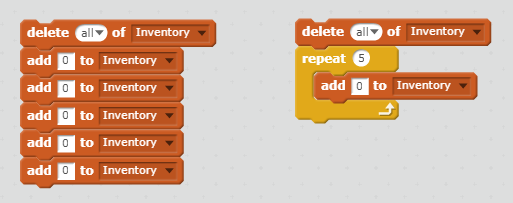
\includegraphics[scale = 0.75]{./Images/Initialize_Inventory.png}
		\end{center}

		
		\item Both methods work but the method on the right is smaller and more concise. Whichever you want to use is fine. Add your method to the bottom of the \textbf{Initialize} block like so:

		\begin{center}
    		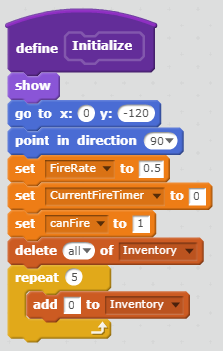
\includegraphics[scale = 0.75]{./Images/XWing_Initialize.png}
		\end{center} 

		\item Now we need something to put into the inventory. What we will be collecting are gems from defeating Tie Fighters. We will now be working in the \textbf{Gem sprite}.
	\end{itemize}
	

	
	
	 

	







\section *{Creating Gems}
	
	\begin{itemize}
		\item I have already provided some skeletal code for us to work off of. 
		\item The \textbf{Clone Event} will contain the behavior for the clones. The \textbf{Spawn Gem} block will handle where the gem clones are spawned. And the \textbf{Pick a Gem} block will handle what kind of gem will be spawned and at what percentage. Continue to work on the \textbf{Clone Event} block until it looks like so:
		\begin{center}
    		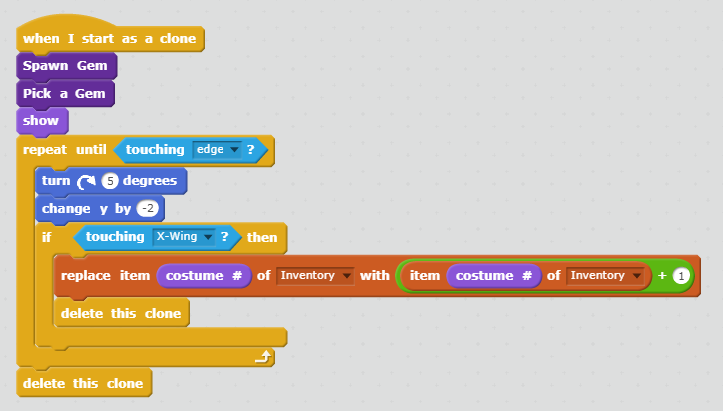
\includegraphics[scale = 0.5]{./Images/Gem_Clone_2.png}
		\end{center}
		\item The way the \textbf{replace item} block works is by associating the gem sprite's costume number to an index in the Inventory list. It then fetches that value and adds 1 to it.
	\end{itemize}



 










\section *{Spawning Gems}

	\begin{itemize}
		\item \hl{Ask the class where they think the gems should spawn in and under what condition (when a tie fighter is destroyed).} 
		\item Proceed to the \textbf{Tie Fighter} sprite. Go to the \textbf{Check if Destroyed} block and show the class where the clone is destroyed. We want to spawn a gem right before the clone is destroyed right where the clone is. But how can we do this? We need the clone's coordinates before it is destroyed. We will save these in lists. \textbf{Create} two lists \textbf{For all Sprites: Gem\_PosX} and \textbf{Gem\_PosY}. 
		\newpage
		\item Add the coordinates of the clone to the appropriate list and spawn a clone of the Gem. Remember, this is the \textbf{Tie Fighter} sprite.

		\begin{center}
			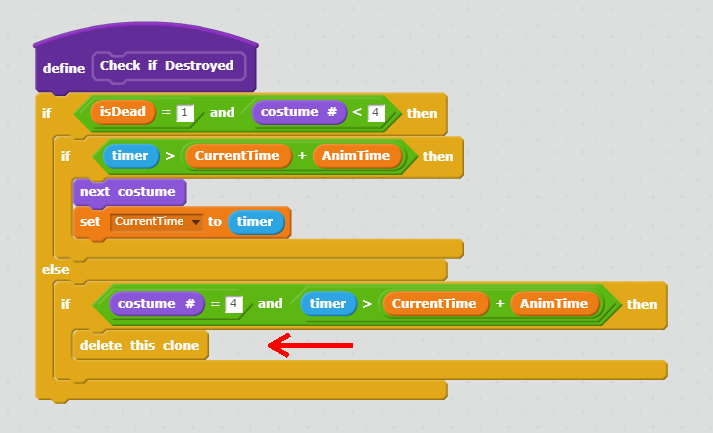
\includegraphics[scale = 0.47]{./Images/TieFighter_CheckDead.png}
		\end{center}

		\begin{center}
			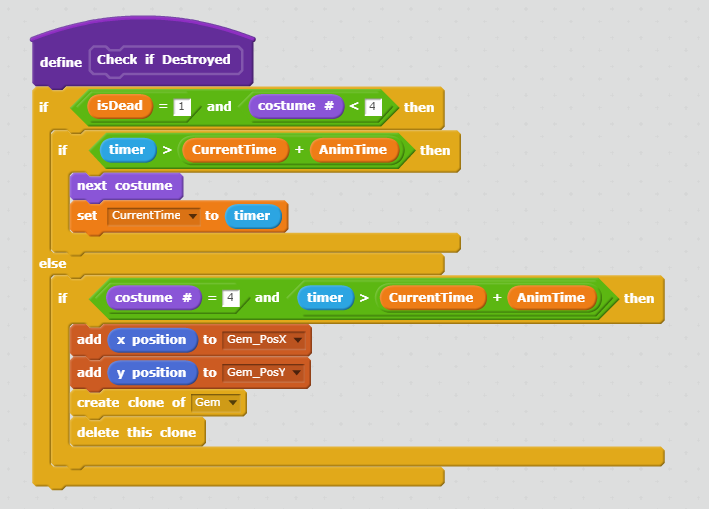
\includegraphics[scale = 0.47]{./Images/TieFighter_CheckDead_2.png}
		\end{center}

		\item We have saved the coordinates for the destroyed tie fighter clone. Now we need to use them. Go to the \textbf{Gem} sprite. Add the following code to the \textbf{Spawn Gem} block:
		\begin{center}
    		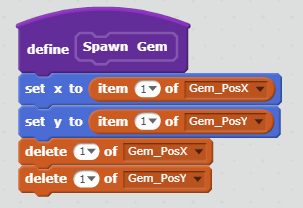
\includegraphics[scale = 0.5]{./Images/Gem_Spawn.png}
		\end{center}
		\item To finish up the \textbf{Gem} sprite, make sure to finish the \textbf{Green Flag Event} by clearing the Gem position lists:
		\begin{center}
    		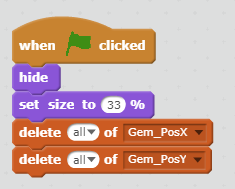
\includegraphics[scale = 0.75]{./Images/Gem_Initialize_2.png}
		\end{center}
		\item \hl{Test it. Make sure the Inventory list is checked so that it shows up in the game. Collecting gems should increment the values in the list.}

	\end{itemize}










\section *{Keeping Score}
	
	\begin{itemize}
		\item Now we are collecting a variety of gems and keeping them in our inventory. Let's give our player a score based on the gems they have collected.

		\item Go to the \textbf{X-Wing} sprite and create a global variable \textbf{PlayerScore}. Add the following code to \textbf{Tally Score} 

		\begin{center}
  			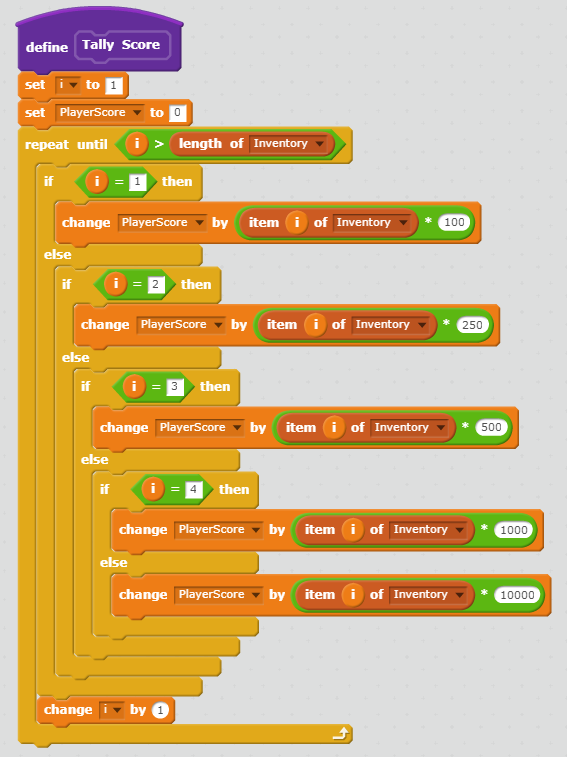
\includegraphics[scale = 0.5]{./Images/XWing_CountScore.png}
		\end{center}
		\newpage
		\item and then the \textbf{Tally Score} block in the \textbf{Green Flag Event} at the bottom but inside the forever loop. Like so:
	
		\begin{center}
  			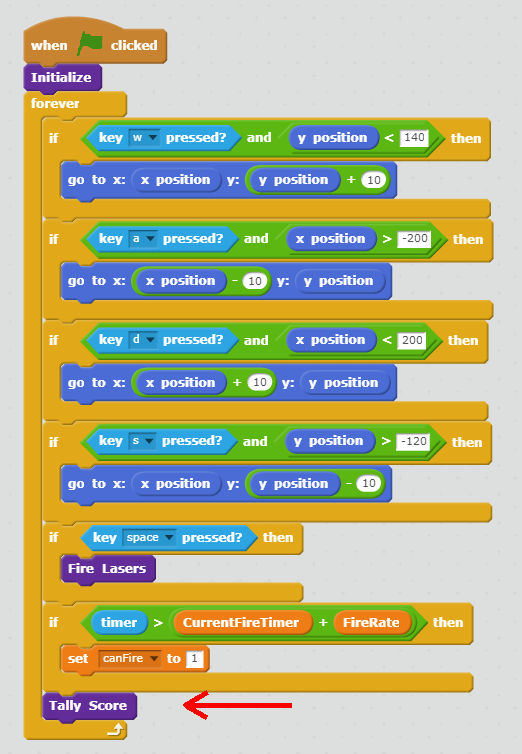
\includegraphics[scale = 0.5]{./Images/XWing_GreenFlag.png}
		\end{center}
	\end{itemize}

		
	
	







\section *{Text Renderer}
	\begin{itemize}
		\item Using Scratch's built in data tracking isn't glamorous and worse, it blocks a lot of our screen when we are playing. Let's integrate someone else's project into our own to be able to render text to the screen and keep track of our score. \\

		\item In a new tab, navigate to Scratch's home page. In the search bar, search for either: \textbf{djpro} or \textbf{Pen Text Engine} and find djpro's pen text engine. Click \textbf{See Inside}, open up your backpack, and drag the first sprite (\textbf{djpro's Text Engine}) into your backpack. This may take a bit of time.\\

		\item Go back to the tab that has your project, make sure it is saved, and refresh it. Open your backpack up and drag the text renderer from your backpack into your sprite section.

		\begin{center}
    		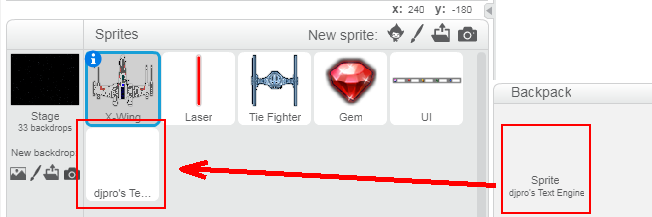
\includegraphics[scale = 0.6]{./Images/djpro.png}
		\end{center}
		\newpage
		\item Find the \textbf{Green Flag Event} (it should be to the right) and delete it and create your own. This is what it should look like:

		\begin{center}
    		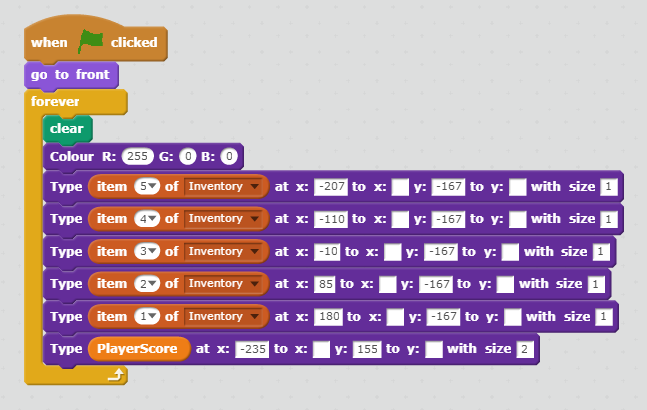
\includegraphics[scale = 0.6]{./Images/TextRenderer_GreenFlag.png}
		\end{center}
	\end{itemize}





\section *{Giving Credit}
	\begin{itemize}
		\item Make sure to credit those who helped you out. In the top right of the the project page, click \textbf{See Project Page} to add your games information and credits. Make sure to include the controls for your game.
	\end{itemize}






\section *{Ideas to Go Further}
	\begin {itemize}
		\item We don't really have a game at the moment, we can't die and there's no real goal to play other than to collect gems. Here are some ideas to take the game to the next level"
		\begin{itemize}
    		\item {Make it so the player can die.}
    		\item {Keep track of waves, maybe add how many waves the player has survived to their score.}
    		\item {Make different kinds of enemies or spawn patterns, or make the enemies shoot their own lasers.}
    		\item {Add power ups and upgrades.}
		\end{itemize}
	\end{itemize}




\end{document}
